\chapter{Analýza metod detekce fyzické aktivity}
\addtocontents{toc}{\protect\setcounter{tocdepth}{1}}

Fyzická aktivita výrazně snižuje koncentraci glukózy v krvi. Z toho důvodu je potřeba před zahájením cvičení snížit dávkování inzulinu, jinak hrozí riziko hypoglykémie. Systémy kontinuální monitorace glukózy jsou sice schopny signalizovat pokles hladiny glukózy, ale tato detekce nemusí nastat včas, nebo není dostatečná. Proto je třeba detekovat parametry fyzické aktivity jako takové.

Většina publikovaných metod využívá k detekci data ze senzorů pro měření srdeční aktivity, teploty kůže, vodivosti kůže a akcelerometrů pro snímání pozice a pohybu těla. Tyto senzory mohou být externí, nebo součástí CGMS.

\section{Metody}
\subsection{The Impact of Accelerometer and Heart Rate Data on Hypoglycemia Mitigation in Type 1 Diabetes}
\label{ch:analyza:PLGS}

\citet{analyzaPA.PLGS} rozšířili existující Predictive low glucose suspend (PLGS) algoritmus. Tento algoritmus predikuje z dat CGM předpokládaný vývoj koncentrace glukózy v krvi a na základě této predikce pozastaví podávání inzulinu inzulinovou pumpou. Snižuje tak riziko hypoglykémie \citep{analyzaPA.PLGS2}.
Pro měření akcelerace a srdečního rytmu použili senzor Zephyr BioHarness 3, k měření glukózy pak Dexcom G4 Platinum CGM nebo Medtronic Sof-Sensor CGM. Predikční okno algoritmu je 30 minut a hranice koncentrace glukózy pro pozastavení podání inzulinu je 80mg/dl. Algoritmus je následně rozšířen tak, aby pozastavil podání inzulinu v případě, že tepová frekvence překročí 90 tepů za minutu, nebo velikost vektoru dat akcelerometru překročí 0,1 a současně koncentrace glukózy v krvi je pod 180 mg/dl.
Pro experiment bylo použito 11 061 měření CGM z čehož 336 bylo pod 70 mg/dl (hypoglykemický stav). Při simulaci bylo zjištěno, že použití samotného PLGS redukuje riziko hypoglykémie o 62 \%. Při použití PLGS v kombinaci s daty akcelerometru a srdečního tepu je redukce 76 \% (viz výsledky v tabulce \ref{tab:analyza:plgs}).

\begin{table}[H]
\caption{Počet hypoglykemických stavů}
\label{tab:analyza:plgs}
\centering
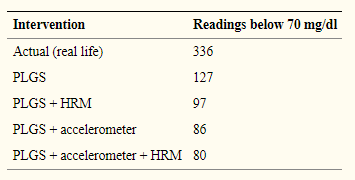
\includegraphics[width=0.6\textwidth]{img/analyzaPA/plgs.png}\\
\textit{Zdroj: The Impact of Accelerometer and Heart Rate Data on Hypoglycemia Mitigation in Type 1 Diabetes \citep{analyzaPA.PLGS}}
\end{table}


\subsection{Physical Activity and Psychological Stress Detection and Assessment of Their Effects on Glucose Concentration Predictions in Diabetes Management}
\label{ch:analyza:SU}

\citet{analyzaPA.SU} využívají strojové učení pro klasifikaci fyzické aktivity. Empatica E4 wristband měří elektrodermální aktivitu, puls, teplotu kůže a akceleraci. Tato data senzor měří každou sekundu. V grafu na obrázku \ref{fig:analyza:su1} je vidět, jak fyzická aktivita ovlivňuje měřená data.

\begin{figure}[H]
\caption{Příklad naměřených dat}
\label{fig:analyza:su1}
\centering
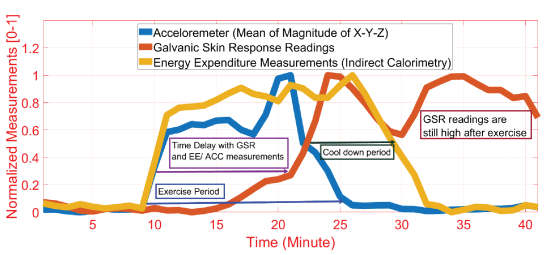
\includegraphics[width=0.9\textwidth]{img/analyzaPA/su1.png}\\
\textit{Zdroj: Physical Activity and Psychological Stress Detection and Assessment of Their Effects on Glucose Concentration Predictions in Diabetes Management \citep{analyzaPA.SU}}
\end{figure}

Z naměřených dat elektrodermální aktivity, teploty a akcelerace byl odstraněn šum pomocí median filtru a Savitzky-Golay filtru. Hodnoty pulsu byli očištěny o šum pomocí Butterworthova band-pass filtru a waveletové dekompozice. Následně se z dat extrahovali charakteristické vlastnosti pro každý minutový interval. Použité parametry jsou uvedeny v tabulce \ref{tab:analyza:su2}. Celkem se extrahovalo 2216 příznaků, z čehož bylo použito 1730 příznaků.

\begin{table}[H]
\caption{Počet hypoglykemických stavů}
\label{tab:analyza:su2}
\centering
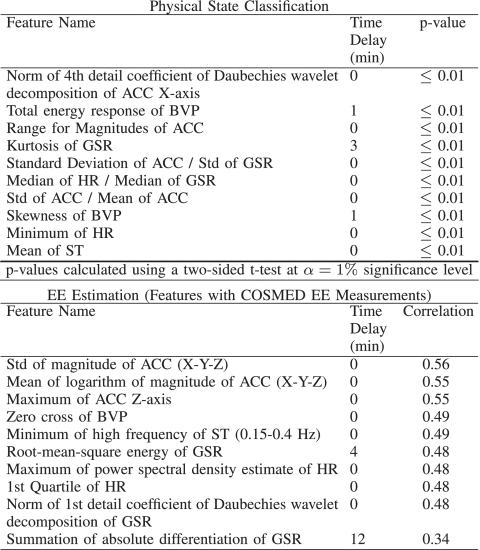
\includegraphics[width=0.8\textwidth]{img/analyzaPA/su2.png}\\
\textit{Zdroj: Physical Activity and Psychological Stress Detection and Assessment of Their Effects on Glucose Concentration Predictions in Diabetes Management \citep{analyzaPA.SU}}
\end{table}

Vysoce korelovaná data moho negativně ovlivnit ptoces strojového učení. Proto bylo použita metoda hlavních komponent (PCA) pro redukci dimenze. Následně byly použity tyto metody strojového učení:
\begin{itemize}
\setlength\itemsep{0em}
\item Long-Short Term Memory (LSTM)
\item Ensemble Learning (EL
\item k-Nearest Neighbors (k-NN)
\item Linear Discrimination/Regression (LD)
\item Naive Bayes (NB)
\item Support Vector Machine/Regression (SVM)
\item Decision Tree (DT)
\end{itemize}

V grafu na obrázku \ref{fig:analyza:su3} je přesnost jednotlivých metod. Nejlépe vychází LSTM s přesností 94,81 \%.

\begin{figure}[H]
\caption{Porovnání jednotlivých metod}
\label{fig:analyza:su3}
\centering
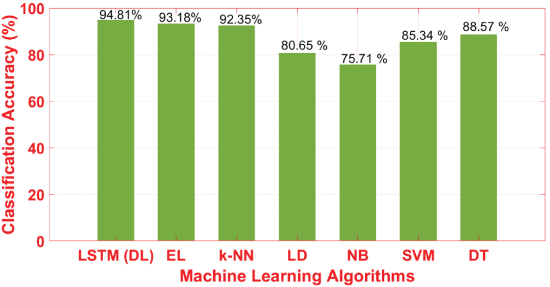
\includegraphics[width=0.8\textwidth]{img/analyzaPA/su3.png}\\
\textit{Zdroj: Physical Activity and Psychological Stress Detection and Assessment of Their Effects on Glucose Concentration Predictions in Diabetes Management \citep{analyzaPA.SU}}
\end{figure}


\subsection{Sensor Monitoring of Physical Activity to Improve Glucose Management in Diabetic Patients: A Review}
\label{ch:analyza:Review}

Autoři této studie \citet{analyzaPA.Review} zjišťovali korelaci mezi koncentrací glukózy v krvi a fyzickou aktivitou. Využli k tomu zařízení SenseWear® Pro Armband vyvinuté firmou BodyMedia (Pittsburgh, PA, USA) pro měření pohybových dat. Toto zařízení je upevněno kolem ruky a sbírá data z pěti typů senzorů. Senzory snímají pozici a pohyb ruky a těla, teplotu kůže a okolí, vodivost kůže a srdeční aktivitu.

Autoři následně použili regresní model pro odhad koncentrace glukózy a zjišťovali korelaci těchto odhadů s daty CGM. Pro experiment, kdy pacienti šli 60 minut po běžeckým pásu, byl korelační koeficient r= 0,90.


\subsection{Black-box Model Identification of Physical Activity in Type-l Diabetes Patients}

V této práci  \citet{analyzaPA.BlackBox} rozšířili  Multi Input Single Output (MISO) black-box model predikce glukózy o data pohybového senzoru. Výsledný model je:


$g(t)=[G_{1}(q^{-1},\theta)G_{2}(q^{-1},\theta)G_{3}(q^{-1},\theta)]
\begin{bmatrix}
i(t)\\
m(t)\\
a(t)
\end{bmatrix}
+H(q^{-1},\theta)e(t)$

kde $g(t)$ je hodnota intersticiální glukózy, $i(t)$ je množství podaného inzulinu, $m(t)$ je množství přijatých karbohydrátů, $a(t)$ je fyzická aktivita a $G_{1}(q^{-1},\theta), G_{2}(q^{-1},\theta), G_{3}(q^{-1},\theta)] a H(q^{-1})$ jsou transfer funkce, kde $q^{-1}[g(t)]=g(t-1)$.

Následující hodnota intersticiální glukózy má rovnici:

$\hat{g}(t|t-1,\theta)=H^{-1}(q^{-1},\theta)[G_{1}(q^{-1},\theta)G_{2}(q^{-1},\theta)G_{3}(q^{-1},\theta)]
\begin{bmatrix}
i(t)\\
m(t)\\
a(t)
\end{bmatrix}\\
\indent +[1-H^{-1}(q^{-1},\theta)]g(t)$

Parametr $\theta$ získáme minimalizováním chyby:

$\hat{\theta} = \operatorname*{arg\,min}_\theta \displaystyle\sum^{N}_{t=1}(g(t)-\hat{g}(t|t-1,\theta))^{2}$

Jako metrika pro vyhodnocení výsledků byly použita střední kvadratická chyba (RMSE) a Koeficient determinace (COD). Porovnání modelu rozšířeného o data fyzické aktivity (I\&M\&A) oproti základnímu modelu (I\&M) v závislosti na délce fyzické aktivity (PH) jsou v grafech na obrázku \ref{fig:analyza:blackbox}. Z grafů je vidět, že pro krátké intervaly si jsou modely podobné, pro delší už I\&M\&A dosahuje lepších výsledků.

\begin{figure}[H]
\caption{Porovnání základního modelu (I\&M) s modelem rozšířeným o data fyzické aktivity (I\&M\&A)}
\label{fig:analyza:blackbox}
\centering
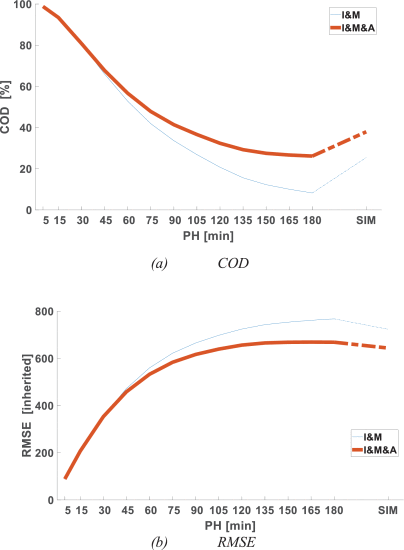
\includegraphics[width=0.7\textwidth]{img/analyzaPA/blackbox.png}\\
\textit{Zdroj: Physical Activity and Psychological Stress Detection and Assessment of Their Effects on Glucose Concentration Predictions in Diabetes Management \citep{analyzaPA.SU}}
\end{figure}


\subsection{A Hybrid Hierarchical Framework for Gym Physical Activity Recognition and Measurement Using Wearable Sensors}
\label{ch:analyza:Weights}

\citet{analyzaPA.Weights} implementovali algoritmus pro detekci fyzické aktivity za pomoci dvou pohybových senzorů. Data akcelerace z obou senzorů jsou nejprve vyhlazena pomocí Savitzky-Golay filtru. Hodnoty tepu jsou získány z EKG senzoru.

V první fázi rozdělí rozdělí aktivity na aerobní cvičení a cvičení se závažím. K tomu použili one-class support vector machine (OC-SVM) klasifikátor. Threshold pro zařazení cvičení do dané kategorie je určen třemi vlastnostmi a to vzdáleností mezi vrcholy, výškou vrcholů a variancí z dat akcelerometrů (rozložení je na obrázku \ref{fig:analyza:weights1}). Přesnost klasifikace je 85 \%.

\begin{figure}[H]
\caption{Rozložení dat akcelerometru podle vzdálenosti mezi vrcholy (růžová), výškou vrcholů (zelená) a variancí (červená)}
\label{fig:analyza:weights1}
\centering
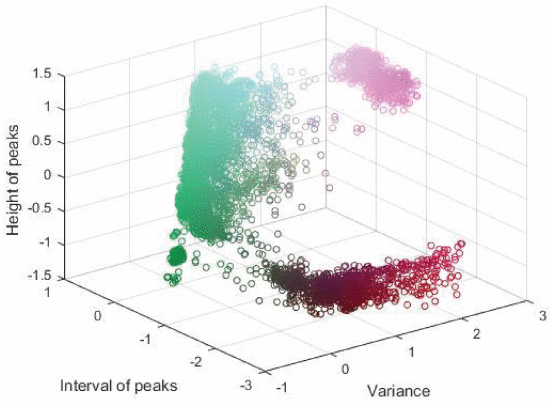
\includegraphics[width=0.8\textwidth]{img/analyzaPA/weights1.png}\\
\textit{Zdroj: A Hybrid Hierarchical Framework for Gym Physical Activity Recognition and Measurement Using Wearable Sensors \citep{analyzaPA.Weights}}
\end{figure}

Následně skrytý Markovův model (HMM) jsou použity pro klasifikaci posilovacích cvičení a neuronové sítě pro klasifikaci aerobních cvičení. U HMM se vychází z toho, že pro určitý cvik se opakuje několik po sobě jdoucích stavů. Pro klasifikaci byl vytvořen soubor stavů a přechodů mezi nimi. Struktura HMM je na obrázku \ref{fig:analyza:hmm}.

\begin{figure}[H]
\caption{Struktura skrytého Markovova modelu}
\label{fig:analyza:hmm}
\centering
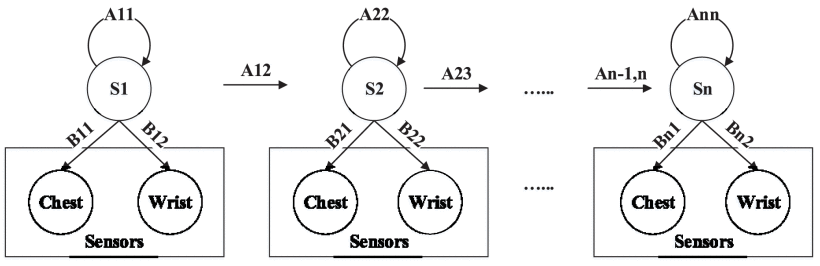
\includegraphics[width=0.8\textwidth]{img/analyzaPA/hmm.png}\\
\textit{Zdroj: A Hybrid Hierarchical Framework for Gym Physical Activity Recognition and Measurement Using Wearable Sensors \citep{analyzaPA.Weights}}
\end{figure}

Přd klsifikací aerobních cvičení se redukuje dimenze dat pomocí metody hlavních komponent (PCA). Nasledně se použije 3 vrstvá neuronová síť. Vstupem vstupní vrstvy jsou data akcelerometru ze zápěstí, skrytá vrstva má 18 a výstupní 9, což odpovídá počtu aerobních aktivit.

Přesnost detekce jednotlivých typů aktivit je mezi 86 \% - 92 \%.


\subsection{Real-Time Recognition of Physical Activities and Their Intensities Using
Wireless Accelerometers and a Heart Rate Monitor}
\label{ch:analyza:NoDiabetes}

\citet{analyzaPA.NoDiabetes} použili pro detekci fyzické aktivity 5 tříosých akcelerometrů a monitor srdečního tepu. Data ze senzorů byly interpolovány cubic spline a rozděleny do posuvného okna po 4,2 sekundách. Pro každé okno pak byla spočítaná plocha pod křivkou, variance, střední hodnota, entropie a korelace pro každou osu. Pro detekci byl použit Naivní Bayesův klasifikátor.

Pro klasifikátor natrénovaný na specifických datech každého jedince byla úspěšnost detekce 94,6 \%. Pro klasifikátor natrénovaný na obecných datech byla úspěšnost detekce pouze 56,3 \%. Podle této studie má srdeční tep pouze malý vliv (1,2 \%) na úspěšnost detekce.




\section{Porovnání metod}

Všechny zkoumané metody využívají k detekci fyzické aktivity alespoň jeden dodatečný senzor. Tyto senzory poskytují data akcelerace ve třech osách. Tato data jsou následně filtrována a jsou získány charakteristické vlastnosti. Část metod pracuje také s daty srdečního rytmu.

Pro klasifikaci dat je následně použita některá z metod strojového učení (kromě metody v kapitole \ref{ch:analyza:PLGS}, kde se požívají pouze thresholdy). Obecně lepších výsledků dosahují metody s tříosým akcelerometrem umístěným na zápěstí. Nejlepší výsledky dosahuje LSTM neuronová síť v kapitole \ref{ch:analyza:SU}. Porovnání metod detekce fyzické aktivity je v tabulce \ref{tab:analyzaPA:res}.

\begin{table}[H]
\caption{Porovnání metod detekce}
\label{tab:analyzaPA:res}
\centering
\begin{tabular}{|l|c|}
\hline 
\textbf{Studie} & \textbf{Úspěšnost detekce}\tabularnewline
\hline 
\hline 
\ref{ch:analyza:SU} \citet{analyzaPA.SU} LSTM & 94,81 \% \tabularnewline
\hline
\ref{ch:analyza:SU} \citet{analyzaPA.SU} EL & 93,18 \% \tabularnewline
\hline
\ref{ch:analyza:SU} \citet{analyzaPA.SU} k-NN & 92,35 \% \tabularnewline
\hline
\ref{ch:analyza:SU} \citet{analyzaPA.SU} LD & 80,65 \% \tabularnewline
\hline
\ref{ch:analyza:SU} \citet{analyzaPA.SU} NB & 75,71 \% \tabularnewline
\hline
\ref{ch:analyza:SU} \citet{analyzaPA.SU} SVM & 85,34 \% \tabularnewline
\hline
\ref{ch:analyza:SU} \citet{analyzaPA.SU} DT & 88,57 \% \tabularnewline
\hline 
\ref{ch:analyza:Weights} \citet{analyzaPA.Weights} & 86 \% - 92 \% \tabularnewline
\hline 
\ref{ch:analyza:NoDiabetes} \citet{analyzaPA.NoDiabetes} specifická data & 94,6 \% \tabularnewline
\hline
\ref{ch:analyza:NoDiabetes} \citet{analyzaPA.NoDiabetes} obecná data & 56,3 \% \tabularnewline
\hline 
\end{tabular}

\begin{flushleft}
Metoda \ref{ch:analyza:PLGS} \citet{analyzaPA.PLGS} není zařazena do porovnání protože autoři neudali počet detekovaných aktivit, ale pouze procentuální snížení počtu hypoglykemických stavů o 76 \%.
\end{flushleft}
\end{table}


\addtocontents{toc}{\protect\setcounter{tocdepth}{2}}